\graphicspath{{figures/research/}}
\chapter{Related Work}\label{ch:related}

\begin{itemize}
	\item object detection
	\begin{itemize}
		\item classification
		\item localisation
	\end{itemize}
	\item deep learning basics
	\item data exploration here?
\end{itemize}

\section{Object Detection}
In order to be able to detect the zebrafish occlusions in every frame, object detection is necessary. Object detection is defined as an employment of computer vision which recognises unique features of objects in an image.

Object detection consists of two main tasks; classification and localisation. It can furthermore be split into two categories depending on the amount of classes which must be detected. If it is only one class, such as detecting humans in an image or detecting any kind of zebrafish occlusion, it is known as class-specific detection. Whereas detecting multiple different kinds of objects is knows as multi-class detection  \citep{Zhang2013}.

The main objective of an object detector is to generate a label list of predefined objects detected in an image. The list should specify which classes are present and where in the image they are located.\\

\todo{Indledning til enten machine- og deep learning, eller blot deep learning]}

\subsection{Machine Learning}
Do we want this??

\subsection{Deep Learning}
Introduce deep learning in general.\\

When using deep learning and a \gls{cnn} for object detection one of the earliest implementations was the \gls{rcnn}. As the name suggests, the method is based upon a region proposal based \gls{cnn} instead of using the often previously used sliding window technique which some times can lead to a large amount of testing windows.

The \gls{cnn} used in the \gls{rcnn} is utilised for feature extraction feeding into a class-specific \gls{svm} to categorise each object. The \gls{cnn} is pre-trained on the ImageNet database and then trained on the PASCAL VOC dataset. An overview of the \gls{rcnn} pipeline is shown in \autoref{fig:rcnn_pipe}

\begin{figure}[h]
	\centering
	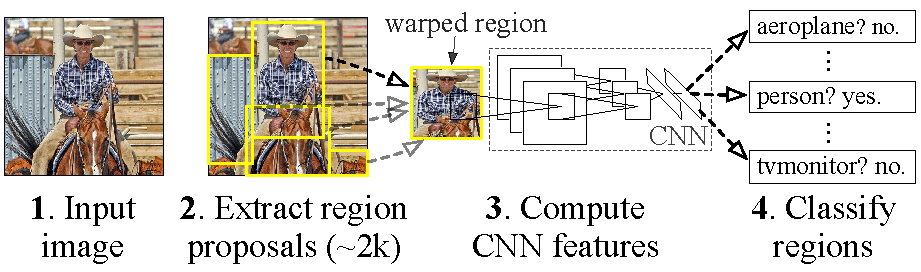
\includegraphics[width=0.9\textwidth]{rcnn_flow}
	\caption{Simple flow diagram of the R-\gls{cnn} by \cite{Girshick2014}}
	\label{fig:rcnn_pipe}
\end{figure}

As shown in \autoref{fig:rcnn_pipe} the \gls{rcnn} is split into 3 individual steps consisting of; region proposals, feature extraction, and \gls{svm} classification.\\

The proposed regions are extracted using \textit{SelectiveSearch} which initialises regions in the image and then merge these with a hierarchical grouping \citep{Uijlings2013}. The final grouping is then a box containing the entire image. The regions are grouped in relation to colour space and similarity \citep{Girshick2014}. 

The next step in the solution is warping the proposed regions to fit the \gls{cnn} input size and extracting features from these and produce a $4096$ dimensional feature vector. The feature vectors consist of both positive and negative proposals found with the SelectiveSearch. These vectors are used to train the class specific \gls{svm}s, one \gls{svm} per class in which a background class is included \citep{Girshick2014}.
When testing a given image, the SelectiveSearch generates approximately 2000 proposals, which each are propagated through the \gls{cnn} to extract feature vectors. Each feature vector is tested against every class-specific \gls{svm}. To remove overlapping detections a greedy Non-maximum Suppression is applied \citep{Girshick2014}.

At the time of publication, the \gls{rcnn} achieves state of the art performance in object detection, with a $~13\%$ increase in precision compared to the previously best method \citep{Girshick2014}.

The \gls{rcnn} does leave room for improvements as it is a slow solution when testing on an image. Furthermore, as the solution is split into multiple modules, the loss calculations for training the \gls{svm}s is not used to update the \gls{cnn}.\\

An improvement on both speed and accuracy of the \gls{rcnn} was published a year later, called Fast \gls{rcnn}. Instead of using the multi module pipeline, as illustrated in \autoref{fig:rcnn_pipe}, training is now done end-to-end. The solution takes an image  and a set of pre-computed object proposals, like the \gls{rcnn} \citep{Girshick2015}.

Instead of individual proposals as in the original \gls{rcnn}, the new iteration propagates the entire image forward through multiple convolutional and max-pooling layers to produce a feature map. The features are extracted from each proposal using a \gls{roi} pooling layer. After the \gls{roi} pooling layer follows two fully connected layers leading to two different outputs; a softmax classification layer and a bounding box regression layer \citep{Girshick2015}. This pipeline is also shown in \autoref{fig:frcnn_pipe}.

\begin{figure}[H]
	\centering
	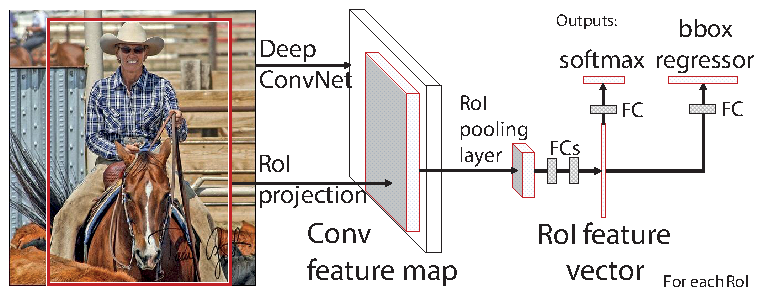
\includegraphics[width=0.9\textwidth]{frcnn_pipe}
	\caption{Fast \gls{rcnn} pipeline overview, by \cite{Girshick2015}}
	\label{fig:frcnn_pipe}
\end{figure}

Just like the \gls{rcnn}, the Fast \gls{rcnn} is pre-trained using the ImageNet database fine tuned for object detection, but instead of being based on AlexNet, as \gls{rcnn} is, the best performing solution of Fast \gls{rcnn} is based on the deeper VGG16 network \citep{Girshick2015}. When comparing to the previous iteration, \gls{rcnn}, it is done while both solutions are using the VGG16 network layout instead of the AlexNet for the \gls{rcnn}. This is done to have a common ground for comparison. Fast \gls{rcnn} improves precision with $4\%$ \citep{Girshick2015}.

The main improvement of the new model is more in speed both in training and testing due to the computing of a convolutional feature map for the entire image. The speed increase is only in relation to the actual detection, as the regions proposals are slow and create a bottleneck for the system \citep{Girshick2015}.\\

To combat the slow region proposals of Fast \gls{rcnn}, \cite{Ren2017} created a third iteration of the \gls{rcnn} network called \textit{Faster \gls{rcnn}}. Here a network named Region Proposal Network (RPN) is implemented to compute region proposals as part of a  network. The RPN shares the convolutional layers and the feature map with the \gls{roi} pooling in the Fast \gls{rcnn}. Due to the layers being computed on the entire image, the time used for proposals generated using the RPN is much lower than of a method such as SelectiveSearch. The RPN, computing region proposals, is the only new part of the Faster \gls{rcnn} compared to Fast \gls{rcnn}.

The results of the Faster \gls{rcnn} in precision are rather small, but the entire computing time of the solution has been significantly minimised, from about $2$ seconds per image to $0.2$ seconds, including region proposals for both timings.

Multiple solutions on the \gls{coco} dataset object detection leader board are still employing the framework of \gls{rcnn} and its predecessors, which shows why the \gls{rcnn} is still a state of the are solution.

%As stated in \autoref{ch:intro}, tracking is dine in multiple different ways and so is the handling of occlusions. The different tracking solutions also enables different approaches to handling the occlusions.
%
%The chapter will focus mainly on solutions which aspire to handle the occlusions in some way, as these may yield the most information towards developing a solution in the project.
%
%\section{Detection}
%Before doing any kind of tracking of the fish in the aquarium, a detection of every object is necessary to be able to gather the required information for tracking. The detection often relies on a high contrast between the desired objects and the background, making the BLOB extraction more simple \citep{Delcourt2018}. The detection step will be defined as the operations made on each frame in a video producing the coordinate of the fish which is then tracked in the following step.\\
%
%According to \cite{Delcourt2018} the detection methods used by multiple different solutions can be dependent on the resolution of the image. Due to identification solutions relying on colour difference between the objects, high resolution images are necessary to be able to properly differentiate between the objects \citep{idtracker2014, Feijo2018, Romero-Ferrero2019}, as the high resolution often leads to each fish being made up of more pixels than in the low resolution images.
%
%When dealing with lower resolution video \cite{Dolado2014} uses a background subtraction from the original image to remove noise in the image. Afterwards a median filter is used to preserve edges and remove the semi-transparent fins of the fish. Lastly segmentation is done converting the image from greyscale to binary using a threshold. Meanwhile, a filter sorts out \gls{blob}s deemed too small to be fish using a size threshold \citep{Dolado2014}.
%
%Similar to \cite{Dolado2014}, \cite{Rodriguez2017} uses a threshold to segment the fish \gls{blob}s from the background image. A size filter is also applied to remove noise and unwanted false positives. Due to the higher resolution data, more information is added to every detection. A square, denoted as a \gls{roi} is drawn around each \gls{blob} and the area is used to generate further information about the \gls{blob}. The information consists of the centre of mass position, the pixel size of the \gls{blob}, a histogram of the \gls{roi} and the time of detection. The information also includes Hu's Seven Moments Invariants, which are used to characterise patterns in images and can be used to identify rigid and moving objects regardless of orientation in the image \citep{Rodriguez2017}.
%
%\cite{idtracker2014} uses a background subtraction which is calculated from the average image of the whole video used for input. As in the other solutions, a threshold is set to segment the \gls{blob}s from the background. To be able to identify each fish in the image, \cite{idtracker2014} collects a set of images of each individual \gls{blob} in the arena. When operating on the video the reference images collected are used to be able to identify each unique \gls{blob} in the image \citep{idtracker2014}.
%
%\cite{Wang2017} and \cite{Pedersen2017} uses head detection of the fish relying on \gls{doh} in scale space with an \gls{svm} classifier to determine if a detection is a fish head or not. \cite{Pedersen2017} utilises \gls{surf} to extract the features of the fish.
%
%\cite{Qian2014} also utilised scale space \gls{doh} \gls{blob} detection, but instead of using an \gls{svm} classifier, extreme points are found and ellipse fitting is done to locate the head of the fish.
%
%\cite{Romero-Ferrero2019} also utilises background subtraction and applies a size dependent filter to eliminate smaller \gls{blob}s, which are not fish, from the image. Furthermore an intensity threshold is used to distinguish the \gls{blob}s from the background.\\
%%Utilising a \gls{cnn}, \cite{Romero-Ferrero2019} is able to detect if two \gls{blob}s are occluding each other.
%
%When detections are made, the tracking is done by connecting the points detected on the fish. This is solved in multiple different ways.
%
%\section{Tracking}
%When successful detections are made, the tracking is to link each detection together for each individual \gls{blob}.\\
%
%
%The low resolution pre processing solution made by \cite{Dolado2014} uses an already commercial tracking solution called \textit{Image-Pro Plus} to track the fish.
%
%A way to connect the desired point on each of the \gls{blob}s is by using the Hungarian algorithm, as done by \cite{Rodriguez2017} and \cite{Pedersen2017}. This is a cost function using the distance between points in two consecutive frames. Both the solutions use the Hungarian algorithm paired with a Kalman filter. The Kalman filter is used to predict the upcoming placement in the following frame, based on previous frames and a state-vector for the fish.
%
%By having identified every fish in the an image, \cite{idtracker2014} are able to track each fish by connecting the centre of mass point of the same identified object in concurrent frame. If a \gls{blob} is recognised as more than one individual, handling of the occlusion is necessary before the tracking can take place.
%
%By using the centre of the fitted ellipse on the fish \cite{Qian2014} uses a state vector consisting of the position and the speed of each individual in $ x $ and $y$ direction. The state vector is used by a Kalman filter to predict the fish's position. To accompany the Kalman filter prediction, \cite{Qian2014} uses feature matching to verify the the predictions made. 
%
%\cite{Wang2017} also uses a Kalman filter prediction paired with a \gls{cnn} based identification to track the fish.
%
%\section{Occlusion Handling}
%During tracking, occlusions can occur and in order to have complete trajectories these must be handled. Some solutions chooses not to handle these and have some missing data points, other solutions handles these occlusions in different manners.
%
%\cite{Dolado2014} uses a single image solution to handle occurring occlusions. They have categorised occlusions into two different types, with two different solutions. By defining a size threshold larger than the observed size of one fish, the \gls{blob}s consisting of two fish or more are segmented in the image. The two different categories of occlusions are an elongation of the fish, making one long \gls{blob}. The other category is when the fish either cross or create a T-like shape \citep{Dolado2014}.
%
%The elongation is handled by eroding the image and then dilating to just before the two \gls{blob}s connect to create only one. To handle the crossing, resulting in an X- or T-shape, an ellipse fitting is made around the \gls{blob} and it is then separated by the shortest axis of the ellipse \citep{Dolado2014}.
%
%\cite{Rodriguez2017} does not state how occlusions are handled, other than when identification is not possible, the \gls{blob} is not assigned to an identification.
%
%By detection the heads of the fish, \cite{Qian2014} are able to distinguish two fish from each other even though a crossing of the bodies occur. If two fish are in a close proximity and a head is close to another fitted ellipse, an angle constraint from the ellipse fitting is applied which is able to differentiate the two and detect the head. Should a head of the fish be occluded, the solution will produce an error and not be able to track the occluded fish at that point. Instead a compensation window of the previous state of the fish is used and the new position of the fish is estimated \citep{Qian2014}. 
%
%\cite{Wang2017} handles occlusions depending on the amount of time the individual is occluded. If the fish is occluded for no more than five consecutive frames, an assumption of the continued predicted path is made based on a constant velocity. If the fish is occluded for longer than five frames, the fish is re-identified by the \gls{cnn} and the trajectory will be missing data from the time it is occluded.
%
%\cite{idtracker2014} has two ways of handling occlusions. Firstly an erosion is attempted as a solution which can often lead to separating two \gls{blob}s from each other. If two individuals are still touching or one is occluding the other, the second step is initiated. Using the identification, the fish which are not in the occlusion are identified, to lower the amount of fingerprints to search for in the occlusion. The average velocity of the fish in the occlusion is found, using the speed of the fish necessary to take part in the occlusion,  if this speed exceeds a threshold, the fish is ruled out. If this does not yield a solution to the issue the individuals are left without an identity.
%
%The newer solution of idtracker, idtracker.ai by \cite{Romero-Ferrero2019} uses a \gls{cnn} to detect occlusions. This network is trained using images of both single animals and occlusions. Then by using the second \gls{cnn} used in th solution, used for identification, is used to identify the two animals taking part in the occlusion. by training the identity network on the images from the data which does not contain occlusions, the identity network is able to identify the animal even though occlusions occur \citep{Romero-Ferrero2019}. It is not mentioned how the solution handles an occlusion of which one individual is completely covered by another.
%
%\todo{Skriv en outro for afsnittet, som skal lede ind i en problem analyse.}